\documentclass[handout]{beamer}
\usepackage[frenchb]{babel}
\usepackage[T1]{fontenc}
\usepackage[utf8]{inputenc}
\usepackage{graphicx}
\usepackage{subfig}
\usepackage{epstopdf}
% functions to plot
\def\func(#1){(#1)*(1-(#1))}
\hypersetup{colorlinks = true,linkcolor = blue,urlcolor  = blue}

\newcommand{\qGraph}[1]{\begin{center} \includegraphics[width =
0.6\textwidth]{#1}\end{center}}

\newenvironment{iPar}[1]{\textbf{#1} \begin{itemize}}{\end{itemize}}

\newcommand{\inc}{{inc}}
\newcommand{\cp}{{cmp}}
\newcommand{\bull}{$\bullet\;$} 

\newcommand{\esp}{\mathbf{E}} \newcommand{\ul}[1]{\underline{#1}}
\newcommand{\ol}[1]{\overline{#1}} \newcommand{\ora}[1]{\textbf{#1}}

\addtobeamertemplate{navigation symbols}{}{%
    \usebeamerfont{footline}%
    \usebeamercolor[fg]{footline}%
    \hspace{1em}%
    \insertframenumber/\inserttotalframenumber
}

\newcommand{\mdp}{\medskip \pause}

\title{Effets Prix et Richesse}
\author{Microéconomie \\ 20851}
\date{}

\begin{document}

\frame{\titlepage}

\section[Outline]{}
\frame{\tableofcontents}

\begin{frame}{Une taxe sur l'essence pousse-t-elle les gens vers le transport en commun?}
\begin{figure}
\subfloat[effet prix]{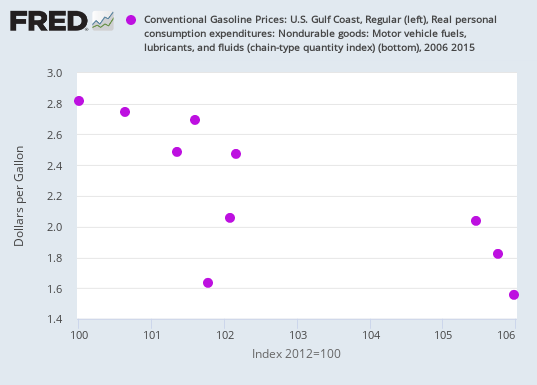
\includegraphics[scale=0.185]{price.png}}
\subfloat[effet revenu]{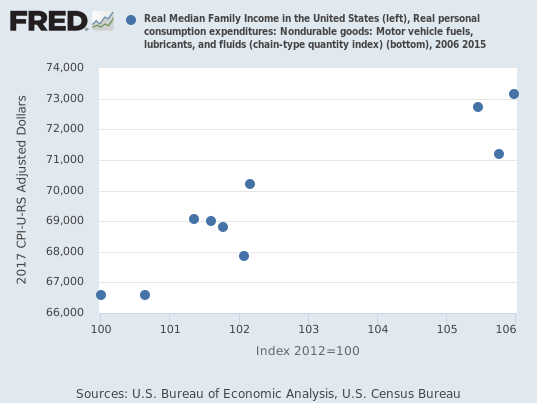
\includegraphics[scale=0.18]{income.png}} 
\subfloat[effet croisé]{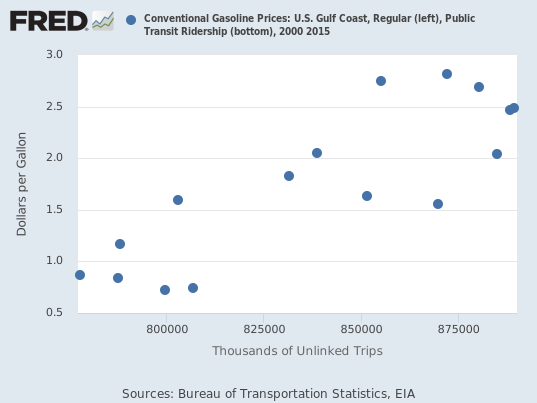
\includegraphics[scale=0.18]{transit.png}}
\caption{FRED Data sur prix, consommation essence et transport en commum}
\end{figure}


\end{frame}

\section{Les variations de prix et de richesse}

\begin{frame}\frametitle{Des préférences à la demande}
\textbf{Le problème}
\begin{itemize}
\item Essence (X) et Tranport en commun (Y)
\item Utilité $U(X,Y)$
\item Contrainte budgétaire: $p_X Y+ p_Y Y = I$
\end{itemize}

\textbf{Optimisation sous contrainte donne:}
\begin{itemize}
\item  $(X^*, Y^*)$ tels que \begin{eqnarray*} \frac{dU}{dX}\Bigg/\frac{dU}{dY} = \frac{p_X}{p_Y} \textrm{ et }
p_X X + p_Y Y = I
\end{eqnarray*}

\item  À l'optimum: contrainte budgétaire respectée, et indifférence entre diminuer un peu de $X$ pour obtenir $Y$ et vice versa.
\item Deux équations, deux inconnus: on peut résoudre pour $X^*$ et $Y^*$ en fonction de $(p_X,p_Y,I)$

\end{itemize}
\end{frame}

\begin{frame}{Exemple}
\begin{itemize}
\item $U(X,Y) = \ln X +  2\ln Y$ \pause
\begin{eqnarray*}\frac{dU}{dX}\Bigg/\frac{dU}{dY} &=& \frac{p_X}{p_Y} \iff \frac{1/X}{2/Y} = \frac{p_X}{p_Y} \\ \iff  p_Y Y = 2p_X X \end{eqnarray*}
\item Avec $p_X X + p_Y Y =  I$ implique $$X^* = \frac{I}{3p_X} \textrm{ et } Y^* = \frac{2I}{3p_Y}$$

\end{itemize}
\end{frame}


\begin{frame}{Comment varient $X^*$ et $Y^*$ en fonction de $I$}
\begin{iPar}{Courbe d'Engel}
\item Demandes individuelles  $X^*(p_X,p_Y,I)$, $T^*(p_X,p_Y,I)$.
\item Courbe d'Engel pour $X$: comment change $X^*$ quand $I$ change
\item Part du budget consacré à $X$: $s_X = \frac{p_X X}{Y}$
\end{iPar} 

\begin{iPar}{Biens normaux}
\item Un bien est normal si et seulement si la demande du bien augmente quand la richesse augmente (prix sont constants)
\item Exemple: essence (voiture de luxe)
\end{iPar}

\begin{iPar}{Biens inférieur}
\item Un bien est inférieur si et seulement si la demande diminue quand la richesse augmente (prix sont constants)
\item Exemple:  dépend du niveau de revenu mais nourriture faible qualité (kraft dinner), billets de loterie, peut-être le transport public?
\end{iPar}

\end{frame}

\begin{frame}{Comment les demandes $X^*$ and $Y^*$ changent avec les prix}
Gardons constants $p_X$ et $p_Y$. Comment la demande répond à une augmentation de $p_X$? 

\end{frame}

\begin{frame}{Décomposition du changement de la demande}
Quand le prix de l'essence $p_X$ augmente, deux forces: \begin{itemize}
\item Transport en commun meilleur affaire que la voiture (essence): Voudra consommer davantage du bien moins cher. C'est l'effet substitution. $$ \frac{U'_X(X,Y)}{U'_Y(X,Y)} = \frac{p_X}{p_Y}$$

\item Le pouvoir d'achat a diminué: besoin de plus de richesse pour acheter le panier avant changement. Effet revenu. $$ dI = Xdp_X + Ydp_Y, dp_X>0 \rightarrow dI<0$$
\end{itemize}

\textbf{Objectif:} Identifier les effets revenu et prix

\end{frame}

\begin{frame}{Demande compensée}

\begin{iPar}{Contexte}
\item Prix de référence $(p_X,p_Y)$, richesse référence $I$, nouveaux prix $(\hat p_X,p_Y)$
\item Demande référence, $X^*(p_X,p_Y,I)$, utilité de référence $V^*(p_X,p_Y,I)$
\item Nouvelle demande, $X^*(\hat p_X, p_Y, I)$, nouvelle utilité $V^*(\hat p_X,p_Y,I)$.
\end{iPar}
\end{frame}

\begin{frame}{Demande compensée}
\begin{iPar}{Définition}
\item Revenu compensée: Revenu $I^\cp$ tel qu'on peut obtenir utilité de référence aux nouveaux prix $$V^*(p_X,p_Y, I) = V^*(\hat p_X, p_Y,  I^\cp)$$
\item Demande compensée $X^\cp = X^*(\hat p_X, p_Y,  I^\cp)$
\item \textbf{Propriété:}  Si $\hat p_X > p_X$, alors $X^\cp <X^*(p_X,p_Y,I)$\\ demande compensée de $X$ est décroissante en $p_X$.
\end{iPar}
\end{frame}

\begin{frame}{Demande compensée}

\textbf{Exercice A}: Calculez le revenu compensé et la demande compensée pour $X$ si $U(X,Y) = XY$ et $p_XX+p_YY \le I$ pour une changement de prix $\hat p_X > p_Y$. 

\end{frame}



\begin{frame}{Effets substitution et revenu}

\begin{iPar}{Effet substitution}
\item  Changement de demande causé par changement de prix relatif, gardant utilité constante
\item Effets substitution $=$ Demande compensée - Demande référence

$$ \Delta X^{\cp} =  X^\cp(\hat p_X,p_Y,I^\cp) - X^*(p_X,p_Y,I) $$

\end{iPar}

\begin{iPar}{Effet revenu}
\item  Changement de demande causé par changement pouvoir d'achat en gardant les prix constant
\item Effet revenu $=$ Nouvelle demande - Demande compensée
\end{iPar}
$$ \Delta X^{I} = X^*(\hat p_X,p_Y,I) - X^\cp(\hat p_X,p_Y,I^\cp) $$

\end{frame}

\begin{frame}{Approximation du revenu compensée}
Considérons petit changement de prix $\hat p_X = p_X + \Delta p_X$. Pour alléger la notation: $X^* = X^*(p_X,p_X,I)$, $Y^* = Y^*(p_X,p_Y,I)$\\ \smallskip

Définissons $I^\cp  = I + \Delta I^\cp$, $X^\cp = X^* + \Delta X^\cp$ and  $Y^\cp  = Y^* + \Delta Y^\cp$.

\begin{align*}
I^\cp & =  \hat p_X X^\cp +  p_Y Y^\cp\\
 & =  (p_X + \Delta p_X)(X^* + \Delta X^\cp) + p_Y(Y^* + \Delta T^\cp)\\ 
  &=  \underbrace{p_X X^* + p_YY^*}_{=I} +\underbrace{\Delta p_X \Delta X^\cp}_{\simeq 0} + \Delta p_X X^* \\
  & \quad \quad \quad + \underbrace{ p_X\Delta X^{\cp} + p_Y \Delta Y^{\cp}}_{=0}\\ & \simeq I+  \Delta p_E E^* \\
 \Delta I^\cp  &\simeq \Delta p_E E^*
\end{align*}
\end{frame}

\begin{frame}{Astuce pour identifier richesse compensée}

Pourquoi $p_X\Delta X^{\cp} + p_Y \Delta Y^{\cp} = 0$?

\begin{enumerate}
\item $(X^*,Y^*)$ et $(X^\cp,Y^\cp)$ sont sur la même courbe d'indifférence, ce qui implique $$\frac{\Delta Y^\cp}{\Delta X^\cp} = TMS_{X\to Y} $$
\item $(X^*,Y^*)$ est optimal aux prix $p_X, p_Y$, ce qui implique $TMS_{X\to Y} = \frac{p_X}{p_Y}$.
\item Donc $p_X \Delta X^\cp + p_Y \Delta Y^\cp = 0 $.
\end{enumerate}

\textbf{Exercice B}: Valider si cette approximation est bonne pour le cas de $U(X,Y) = XY$ et les prix, revenu de référence sont $(p_X,p_Y,I) = (1,1,100)$ et $\Delta p_X = 1$, $\Delta p_X = 0.1$.
\end{frame}

\begin{frame}{L'équation de Slutsky}
Cette équation vient de la décomposition de l'élasticité de la demande par rapport aux prix.\medskip

Pour alléger la notation, considérons 
\begin{align*}
 X^* &= X^*(p_X,p_Y,I), &     X^*(p_X + \Delta p_X, p_Y,I) &= X^* + \Delta X^*,\\ && X^*(p_X + \Delta p_X, p_Y,I) &= X^\cp +\Delta X^I
\end{align*}

Nous obtenons
\begin{align*}
\underbrace{\Delta X^*}_{\text{Effet total}} = \underbrace{\Delta X^\cp}_{\text{Effet substitution}} + \underbrace{\Delta X^I}_{\text{Effet revenu}}
\end{align*}

\textbf{Exercice D}: Calculer ces effets substitutions et revenu dans le cas de l'exercice C.
\end{frame}


\begin{frame}{L'équation de Slutsky}
Puisque $$\Delta X^I =   -\frac{\partial X}{\partial I} \Delta I^\cp =  -\frac{\partial X}{\partial I}  \Delta p_X X^*$$
Alors,
\begin{align*}
\Delta X^* &=   \underbrace{\Delta X^{\cp}}_{\leq 0} -   \underbrace{\frac{\partial X}{\partial I}\times \Delta p_X X^*}_{\geq 0 \text{ si normal, } <0 \text{ si inférieur}} 
\end{align*}
En forme d'élasticité, 
\begin{align*}
\frac{\Delta X^*}{\Delta p_X}\frac{p_X}{X^*} & = \frac{\Delta X^\cp}{\Delta p_X}\frac{p_X}{X^*} - \frac{\partial X}{\partial I} \Delta p_X X^*\times\frac{p_X}{\Delta p_X X^*}\frac{I}{I} 
\end{align*}
L'équation de Slutsky est donnée par: 

$$\eta_{X,p} & = \eta^\cp_{X,p}  - \eta_{X,I} \times s_X $$

\end{frame}

\section{Propriétés des fonctions de demande}

\begin{frame}{Nature des biens}

Les biens $X$ et $Y$ sont:
\begin{itemize}
\item Substituts: si l'effet prix croisé $\frac{\partial X^\cp}{\partial p_Y} >0$
\item Compléments: si l'effet prix croisé $\frac{\partial X^\cp}{\partial p_Y} <0$ 
\end{itemize}

\end{frame}

\begin{frame}{Propriétés}

\begin{itemize}
\item Homogénéité de degré 0 $$X(\lambda p_X,\lambda p_Y,\lambda I) = X(p_X,p_Y,I)$$ 
\item Symétrie: $$\frac{\partial X^\cp}{\partial p_Y} =\frac{\partial Y^\cp}{\partial p_X} $$ 
\item Additivité: $$ p_X \frac{\partial X(p_X,p_Y,I)}{\partial I} + p_Y \frac{\partial Y(p_X,p_Y,I)}{\partial I} = 0 $$
\item Négativité: $$\frac{\partial X^\cp}{\partial p_X}<0,\frac{\partial Y^\cp}{\partial p_Y}<0$$

\end{itemize}

\end{frame}

\section{Cas particuliers}

\begin{frame}{Biens Giffen}
\begin{iPar}{Direction des effets revenus et richesses}
\item Quand courbes indifférence convexes, demande compensée pour $E$ diminue quand $p_E$ augmente
\item Effet richesse dépend si bien est inférieur ou normal aux prix et richesse de référence.
\item Si bien normal, augmentation de prix donne effet richesse négatif (même sens que effet prix)
\item Si bien inférieur, augmentation du prix génère effet richesse positif (sens contraire)
\end{iPar}

\begin{iPar}{Biens Giffen}
\item Si effet richesse plus grand qu'effet substitution, quand prix $p_E$ augmente, demande pour $E$ augmente.
\item  Exemple classique : Pommes de terre en Ireland (vers 1850, selon la légende). 
\end{iPar}
\end{frame}

\begin{frame}{Subvention aux pauvres en Chine}

\begin{figure}
\subfloat{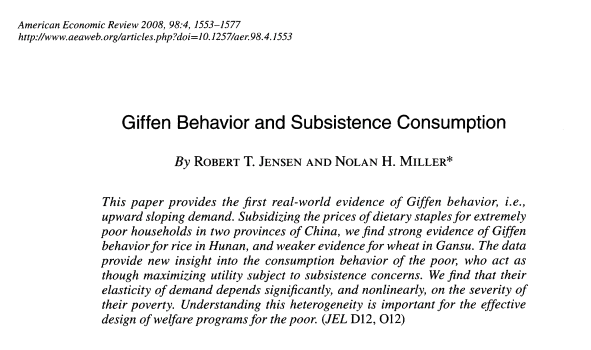
\includegraphics[scale=0.3]{china.png}}
\subfloat{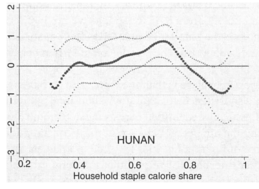
\includegraphics[scale=0.5]{elasticity_share.png}}
\end{figure}

\end{frame}

\begin{frame}{Les médecins}
Comment une hausse du salaire peut faire diminuer le nombre d'heures?
\begin{figure}
\centering

\includegraphics[scale=0.2]{docteurs.png}
\caption{\href{https://www.tvanouvelles.ca/2018/05/17/medecins-de-familles-la-moitie-travaillent-4-jours-et-moins}{TVA Nouvelles}}
\end{figure}
\end{frame}

\begin{frame}{Les indices de prix et coût de la vie}

Pour mesurer les changements de coût de la vie, on utilise souvent les indices de prix à la consommation. Un très utilisé est l'indice de Laspeyres: 

$$ \pi_L = \frac{\hat p_X X + \hat p_Y Y}{p_X X + p_Y Y} $$

\begin{itemize}
\item Le Régime des rentes du Québec mais aussi les régimes privés sont (souvent) indexés à un indice de ce type. 
\item Est-ce que ceci est un bon indice de la hausse du coût de la vie?

\end{itemize}

\end{frame}

\begin{frame}{Indice de prix idéal}

Les comportements changent. Donc une hausse de prix implique de la substitution. 

\begin{itemize}
\item Suivant une hausse de prix au bien $x$, la compensation nécessaire pour garder le bien-être constant est 

$$ \pi_I =  \frac{I^{cmp}}{I} $$.

\item Dans le cas Cobb-Douglass $u(x,y)=x^{\alpha}y^{1-\alpha}$: 

$$ \pi_I = \frac{I^{cmp}}{I} = \left(\frac{\hat p_X}{p_X}\right)^\alpha$$

\end{itemize}

\end{frame}

\end{document}




